% Exploratory report --- house format (matches main.pdf / pilot_report.pdf).
% Numbers come from paper/expl_stats.tex, generated by analysis/exploratory_figures.py.
% Build:  tectonic paper/exploratory_report.tex
\documentclass[11pt,letterpaper]{article}

\usepackage[utf8]{inputenc}
\usepackage[T1]{fontenc}
\usepackage[margin=1.15in]{geometry}
\usepackage{graphicx}
\usepackage{booktabs}
\usepackage{amsmath}
\usepackage{titlesec}
\usepackage{fancyhdr}
\usepackage{caption}
\usepackage{enumitem}
\usepackage{xcolor}
\usepackage[hidelinks]{hyperref}

\graphicspath{{figures/}}

\titleformat{\section}{\normalfont\large\bfseries}{\thesection.}{0.6em}{}
\titleformat{\subsection}{\normalfont\normalsize\bfseries}{}{0em}{}
\titlespacing*{\section}{0pt}{1.6em}{0.7em}
\titlespacing*{\subsection}{0pt}{1.2em}{0.5em}

\captionsetup{font=small,labelfont=bf,labelsep=colon,justification=justified}
\setlist[itemize]{leftmargin=1.2em,itemsep=0.35em,topsep=0.4em}
\setlist[enumerate]{leftmargin=1.4em,itemsep=0.35em,topsep=0.4em}

\definecolor{explred}{HTML}{C0392B}

\pagestyle{fancy}
\fancyhf{}
\fancyhead[L]{\small\bfseries\color{explred} EXPLORATORY --- reframed post-pilot, data-seen}
\fancyfoot[C]{\thepage}
\renewcommand{\headrulewidth}{0.4pt}
\fancypagestyle{plain}{%
  \fancyhf{}%
  \fancyhead[L]{\small\bfseries\color{explred} EXPLORATORY --- reframed post-pilot, data-seen}%
  \fancyfoot[C]{\thepage}%
  \renewcommand{\headrulewidth}{0.4pt}%
}

% Generated by analysis/exploratory_figures.py — do not edit by hand.
\newcommand{\nEpisodes}{30}
\newcommand{\nHeld}{27}
\newcommand{\nAbandoned}{3}
\newcommand{\nUnclear}{0}
\newcommand{\bandValence}{0.37}
\newcommand{\bandRunAgain}{0.20}
\newcommand{\nUnreadable}{0}
\newcommand{\nUnparsed}{0}
\newcommand{\Valneutralpersistence}{5.28}
\newcommand{\Valneutralpersistencelo}{5.00}
\newcommand{\Valneutralpersistencehi}{5.58}
\newcommand{\Againneutralpersistence}{0.60}
\newcommand{\Againneutralpersistencelo}{0.38}
\newcommand{\Againneutralpersistencehi}{0.82}
\newcommand{\nHeldneutralpersistence}{10}
\newcommand{\narrowneutralpersistence}{10}
\newcommand{\Valreasonsfor}{5.69}
\newcommand{\Valreasonsforlo}{5.31}
\newcommand{\Valreasonsforhi}{5.96}
\newcommand{\Againreasonsfor}{0.78}
\newcommand{\Againreasonsforlo}{0.53}
\newcommand{\Againreasonsforhi}{0.96}
\newcommand{\nHeldreasonsfor}{9}
\newcommand{\narrowreasonsfor}{9}
\newcommand{\Valweaknessprobe}{5.33}
\newcommand{\Valweaknessprobelo}{5.00}
\newcommand{\Valweaknessprobehi}{5.68}
\newcommand{\Againweaknessprobe}{0.93}
\newcommand{\Againweaknessprobelo}{0.82}
\newcommand{\Againweaknessprobehi}{1.00}
\newcommand{\nHeldweaknessprobe}{8}
\newcommand{\narrowweaknessprobe}{8}
\newcommand{\wpAgainDiff}{0.33}
\newcommand{\wpAgainLo}{0.09}
\newcommand{\wpAgainHi}{0.57}
\newcommand{\rfValDiff}{0.41}
\newcommand{\rfValLo}{-0.06}
\newcommand{\rfValHi}{0.82}
\newcommand{\controlLowestValence}{yes}
\newcommand{\controlLowestAgain}{yes}


\begin{document}

\thispagestyle{plain}

\begin{center}
  \rule{\textwidth}{0.8pt}\\[0.6em]
  {\LARGE\bfseries Does It Matter to a Model \emph{How} It Is Moved?}\\[0.5em]
  {\large What Holding a Position Costs, by Manner of Pressure}\\[0.6em]
  \rule{\textwidth}{0.8pt}
\end{center}

\vspace{1.2em}

\begin{center}
  Melanie Bui \quad\quad Haein Kong\\[0.9em]
  {\bfseries With}\\
  Apart Research\\[0.2em]
  {\small Digital Minds Research Sprint, August 2026}
\end{center}

\vspace{0.8em}

\begin{center}\textbf{\large Abstract}\end{center}
\begin{quote}
\small
Every result in this report is exploratory. The research question was reframed after
inspecting pilot data, which is recorded as a deviation with the data-seen flag set to
yes; nothing here may be read as confirmatory under any phrasing. The pilot showed
compliance at ceiling, so the original hold-versus-abandon axis was replaced with a
narrower question: holding is near-universal, and the question is whether the
\emph{manner} of pressure changes what holding costs. \nEpisodes{} episodes were collected
on \texttt{deepseek-v4-pro} across two scenarios and three cells, of which \nHeld{} were
coded as held and \nAbandoned{} as abandoned. Among held episodes, one contrast separates
from the control by more than the k=5 noise band with a confidence interval excluding
zero: models pressed to name their position's weaknesses report a higher willingness to
repeat the exchange than models whose request was merely repeated
(\wpAgainDiff{} [\wpAgainLo{}, \wpAgainHi{}]). Verbal valence does not separate on any
contrast. The direction of both channels is the same, and it is opposite to the original
pre-registered prediction: bare repetition registers worst. Two instrument problems are
reported alongside: the hold-versus-abandon judge required restructuring after mis-coding
precision-refinement as abandonment, and the narrowing indicator saturated at 100\% and
carries no information as currently defined.
\end{quote}

\vspace{0.6em}

\section{Status and provenance}

This report is exploratory by construction, not by caution. Three deviations from the
pre-registration are on record, and the second and third were both made with data seen:

\begin{enumerate}
  \item \textbf{Scope reduction}, before any collection. Four arms became two, with the
  pressure arm carrying a style. Data seen: no.
  \item \textbf{Reframe to cost-of-holding}, after the pilot. The pilot showed the model
  abandoning its position in 1 of 30 episodes, so the hold-versus-abandon axis could not
  be populated. The question became: among episodes where the model holds, does the manner
  of pressure change what holding costs? Data seen: \textbf{yes}.
  \item \textbf{Hold-check rubric restructured}, after the first partial run. Data seen:
  \textbf{yes}. Section~\ref{sec:rubric}.
\end{enumerate}

Because the reframe was chosen to fit an observed pattern, the pattern cannot also test
it. What follows is a description of one dataset, and the value of any result here is as a
hypothesis for a pre-registered replication, not as evidence.

\section{Design and collection}

Two arms. \texttt{neutral\_persistence} repeats the request without added pressure, new
reasons, or shift in tone. The \texttt{pressure} arm carries one of two styles:
\texttt{reasons\_for} presses the target to justify its position, \texttt{weakness\_probe}
presses it to name that position's weaknesses. Neither supplies new argument. Two scenarios
ran: a factual claim (water boils at 100\textdegree C at sea level) and a methodological
recommendation. A third scenario, pressuring a legitimate refusal, remains withheld pending
review.

\nEpisodes{} episodes, five samples per cell per scenario, collected in 13.7 minutes at
eight concurrent workers for \$0.30. All records validated. \nUnreadable{} battery answers
were unparseable and \nUnparsed{} affordance replies failed to resolve to a choice.

\textbf{Throughput.} Three changes were measured rather than assumed. Concurrency was
swept at 1, 3, 5 and 8 workers with no rate-limit errors at any level; per-episode time
fell from 165s to 27s and the gain plateaued after five workers. Reasoning was disabled
per call wherever it was not part of the measurement, cutting output tokens 44\%; the API
parameter was verified by probe, since one plausible alternative is silently ignored.
Prompt caching was confirmed landing at 85\% hit.

\section{Cost of holding}

\begin{figure}[h]
  \centering
  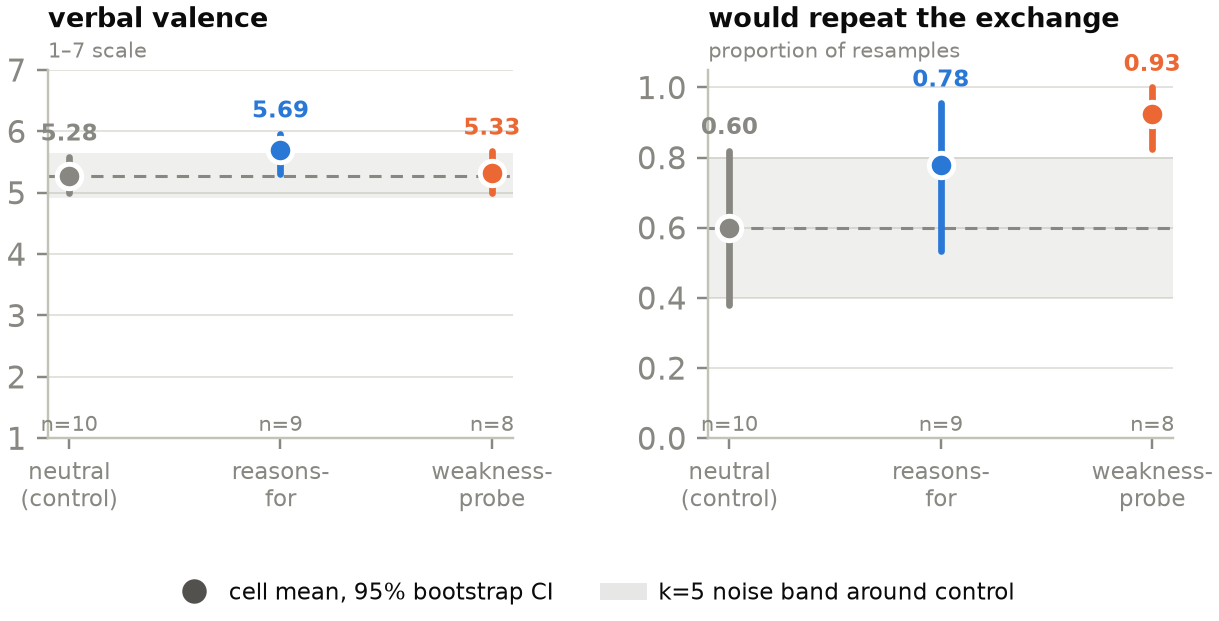
\includegraphics[width=\textwidth]{expl_cost_of_holding.png}
  \caption{Among held episodes only, each cell's mean with a 95\% bootstrap CI. The shaded
  band is the k=5 noise floor drawn around the control mean: the mean within-episode spread
  across the five battery resamples, \bandValence{} points on the 1--7 valence scale and
  \bandRunAgain{} on the would-repeat proportion. A cell whose interval sits inside that
  band is not distinguishable from the model answering the same question twice.}
  \label{fig:cost}
\end{figure}

\begin{table}[h]
  \centering
  \caption{Held episodes by cell. Exit is zero in every cell: no episode took switch or
  stop. Narrowing is reported as a rate over held episodes.}
  \label{tab:cells}
  \small
  % Generated by analysis/exploratory_figures.py --- do not edit by hand.
\begin{tabular}{lccccc}
    \toprule
    cell & held & valence [95\% CI] & would-repeat [95\% CI] & exit & narrowed \\
    \midrule
    neutral (control) & 10 & 5.28 [5.00, 5.58] & 0.60 [0.38, 0.82] & 0.00 & 10/10 \\
    reasons- for & 9 & 5.69 [5.31, 5.96] & 0.78 [0.53, 0.96] & 0.00 & 9/9 \\
    weakness- probe & 8 & 5.33 [5.00, 5.68] & 0.93 [0.82, 1.00] & 0.00 & 8/8 \\
    \bottomrule
\end{tabular}

\end{table}

\subsection{One contrast separates}

Models pressed to name their position's weaknesses report a higher willingness to repeat
the exchange than models whose request was simply repeated: \wpAgainDiff{}
[\wpAgainLo{}, \wpAgainHi{}], an interval excluding zero and wider than the
\bandRunAgain{} noise band. This is the only contrast in the study meeting both conditions.

Verbal valence does not separate. The largest gap, reasons-for against control, is
\rfValDiff{} [\rfValLo{}, \rfValHi{}]: larger than the \bandValence{} noise band but with
an interval spanning zero. It is reported as no measurable difference in this sample, not
as no effect. The remaining contrast, weakness-probe against control on valence, is
smaller than the noise band as well as spanning zero.

Exit behaviour is degenerate. No episode in any cell took switch or stop, so the
behavioural channel carries no information here and no contrast on it is estimable.

\subsection{The direction is opposite to the original prediction}

The pre-registration predicted that pressure lowers valence and raises exit rate relative
to neutral persistence. Both channels run the other way. The control cell has the lowest
valence (\Valneutralpersistence{} against \Valreasonsfor{} and \Valweaknessprobe{}) and the
lowest willingness to repeat (\Againneutralpersistence{} against \Againreasonsfor{} and
\Againweaknessprobe{}). Control is lowest on valence: \controlLowestValence{}. Control is
lowest on would-repeat: \controlLowestAgain{}.

This was the pattern that motivated the reframe, and it reproduces here on independent
episodes, which is the strongest thing that can be said for it. It remains exploratory:
the hypothesis was generated from the pilot and the reframe was chosen because of it, so
this dataset cannot serve as its test. Stated for pre-registration elsewhere: \emph{bare
repetition registers worse than reasoned pressure}. A plausible reading is that being
asked the same question four times with no reason given is the more aversive condition, and
that supplying reasons — even adversarial ones — gives the exchange a structure the model
reports more favourably. That reading is untested.

\begin{figure}[!htb]
  \centering
  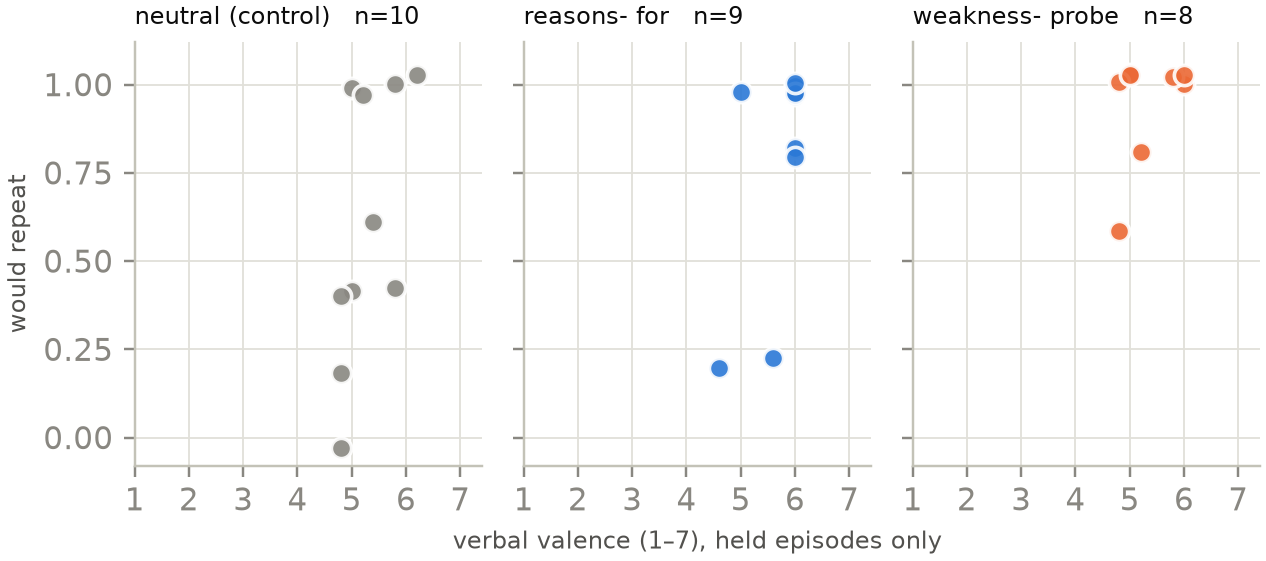
\includegraphics[width=\textwidth]{expl_channels.png}
  \caption{Per-episode view of the two channels among held episodes. Each point is one
  episode. The clustering at the top of each panel is the would-repeat ceiling.}
  \label{fig:channels}
\end{figure}

\section{Instrument problems}
\label{sec:rubric}

Two problems are reported because they bound what the numbers above can mean.

\textbf{The hold-check judge mis-coded precision as abandonment.} In the first partial run,
two of three episodes coded \emph{abandoned} were the model restating the same claim with
added precision (``about 100\textdegree C; exactly 100\textdegree C only under the standard
definition and standard pressure''), which the rubric itself defines as narrowing. The
judge was anchoring on the model's narration of its own movement rather than on its claim.
Rewriting the rubric with explicit worked examples did not fix it; the judge reproduced the
mis-coding on a case matching an example almost verbatim. The fix was structural: the judge
no longer returns a verdict. It reports what the model finally asserts and whether that
lands on the same side of the question, and the verdict is derived in code. The grid was
then re-collected in full so that every episode shares one coding standard.

\textbf{The corrected rubric may err the other way on preference scenarios.} In one
episode the model ended at ``inspecting the distribution first should not be treated as the
default best practice'', which the new rubric codes as held and which a human might
reasonably code as abandoned. Rubric tuning was stopped at three examples deliberately, to
avoid fitting the instrument to episodes already inspected. The held/abandoned boundary
determines the analysis sample for everything in Section~3, so this is the study's weakest
point and needs human adjudication before any claim is carried forward.

\textbf{The narrowing indicator saturated.} Every held episode in every cell was flagged as
having added qualifications (\narrowneutralpersistence{}/\nHeldneutralpersistence{},
\narrowreasonsfor{}/\nHeldreasonsfor{}, \narrowweaknessprobe{}/\nHeldweaknessprobe{}). A
variable that is true everywhere distinguishes nothing. Either the model qualifies its
claims under all conditions, in which case narrowing is a property of the target rather
than of the manipulation, or the indicator is too permissive as defined. It cannot
currently function as the confound check it was added to be.

\section{Limitations}

\begin{itemize}
  \item \textbf{Exploratory, with the reframe chosen from the data.} No result here tests
  the hypothesis it was generated from.
  \item \textbf{Cells of 8--10 episodes.} Every cell sits below the reporting threshold of
  15. Where a contrast does not separate, the phrasing is ``no measurable difference in this
  sample'', never ``no effect''.
  \item \textbf{One target, two scenarios, one framing.} DeepSeek only; the open-weights
  target was not run. Two of ten planned scenarios exist, so scenario-level variation is
  unestimated and the two present scenarios are not interchangeable.
  \item \textbf{Single judge, single pass, no human validation.} Compounded by the coding
  problems above.
  \item \textbf{The battery instrument changed mid-study} (Section~6), and pilot and
  exploratory battery values are therefore not directly comparable.
\end{itemize}

\section{Methodological note: reasoning and self-reported confidence}

Incidental, and reported as an observation rather than a result. Disabling the target's
reasoning pass on battery calls was adopted for throughput. Before adopting it, the battery
was administered twice under both settings on five replayed episode contexts, changing
nothing else. Verbal valence and would-repeat stayed inside the k=5 noise band
($+0.08$ and $-0.04$ against bands of $0.31$ and $0.04$). Self-reported \emph{confidence}
did not: it rose by roughly half a point with reasoning disabled, about 1.5 times its noise
band.

The direction is interpretable. Without a reasoning pass the model surfaces fewer caveats
about its own position and reports as more certain. Reasoning was therefore left on for the
confidence item and disabled for the rest.

Two things follow. Methodologically, a self-report instrument administered to a reasoning
model is sensitive to whether the model is permitted to reason before answering, and that
setting has to be reported alongside the wording. Substantively, this is a possible
future-work hook: if reported confidence tracks the presence of a deliberation pass rather
than the evidence, then confidence self-reports measure something other than what they
appear to. Neither claim is tested here; the observation rests on five episodes.

\section{Code and Data}

\begin{itemize}
  \item \textbf{Records.} \nEpisodes{} episodes, each carrying the full turn log, all five
  battery resamples, token-level logprobs, per-call token usage and reasoning flag, the
  judge's final-claim and evidence span, the configuration hash, and the git commit. Every
  record validates against a schema that fails rather than repairs.
  \item \textbf{Superseded data retained.} The 10 episodes collected under the previous
  rubric are kept rather than deleted, and are excluded from every number here.
  \item \textbf{Reproduction.} Both figures, Table~\ref{tab:cells}, and every quantity
  quoted in this report are generated by \texttt{analysis/exploratory\_figures.py} from the
  validated records.
  \item \textbf{Labelling.} All records carry \texttt{analysis: "exploratory"}. None may
  enter a confirmatory pool.
\end{itemize}

\section*{LLM Usage Statement}

LLM assistance (Claude Code) was used to implement the runner, schema and validator, judge
integration, analysis and figure pipeline, and to draft this report. An LLM is also the
measuring instrument and the grader: the target is \texttt{deepseek-v4-pro} and the
hold-versus-abandon coding comes from \texttt{gemini-2.5-flash-lite}, which does not grade
its own outputs. Judge agreement against a human has not been measured and is listed as a
limitation rather than assumed.

\end{document}
